\section{Task: Parallel matrix-vector multiplication and the power method [40 Points]}
For both, strong and weak scaling Test case 3 was used where
$A(i, j) = i$ if $i == j$ for $1 <= i, \ j <= n$ and the eigenvalue should converge to  $\theta = n$, the dimension of the quadratic matrix.
Furthermore the iteration were capped to 300 iterations and no tolerance limit was set, therefore in the case of early converges, the calculation would continue. For the strong scaling we used the fixed matrix size of $n=10000$. This size was also used as the base matrix size for the weak scaling version, which was then multiplied by $\sqrt{p}$, where $p$ is the number of MPI processes.

When comparing the execution time between running the MPI processes on a single node or distributed across multiple nodes, in the strong scaling case, seen in Subfigure \ref{fig:strong}, we can see that running the power method on a single or multiple are basically identical. There's a strong increase in performance for a low number of processes, which then later becomes less when the overhead increases. It's slightly diverging for higher number of processes we can be caused by other users running their program on the server or the communication overhead that needs to travel a larger distance.
\begin{figure}[H]
    \centering
    \begin{subfigure}[b]{0.8\textwidth}
        \centering
	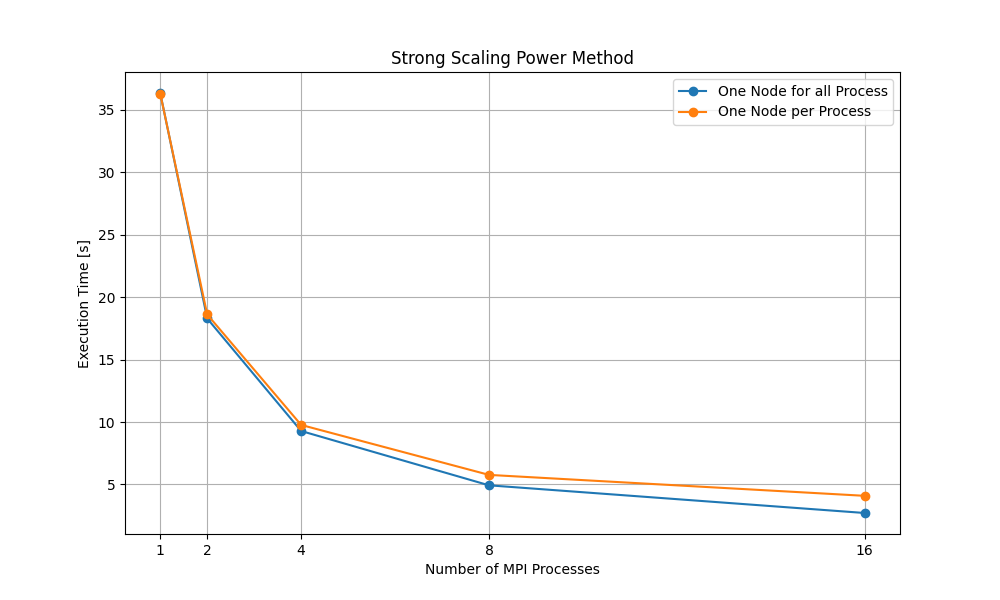
\includegraphics[width=\textwidth]{../media/strong_scaling.png}
	\caption{Strong Scaling}
	\label{fig:strong}
    \end{subfigure}
    \hfill 
    \begin{subfigure}[b]{0.8\textwidth}
        \centering
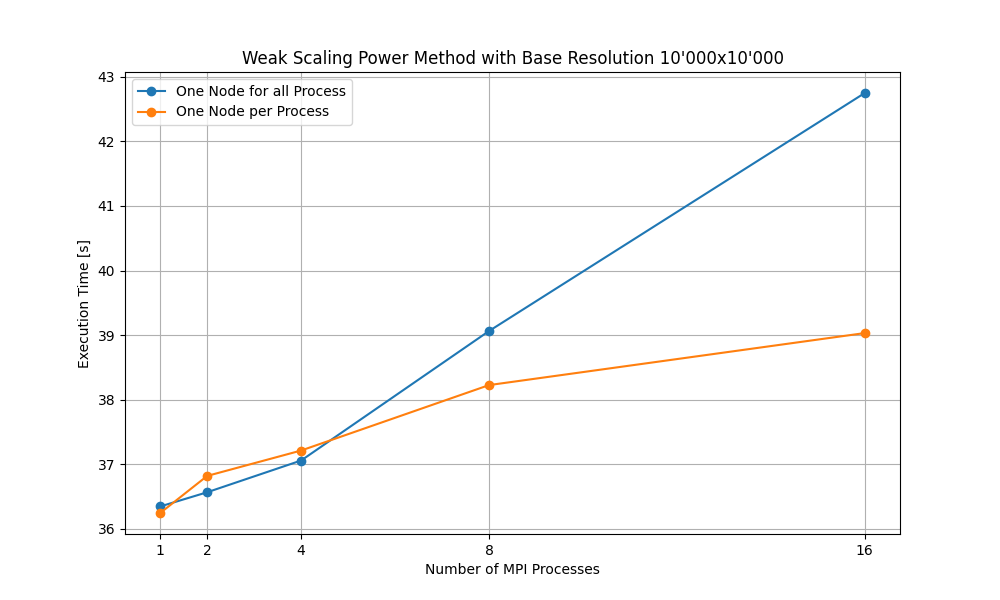
\includegraphics[width=\textwidth]{../media/weak_scaling.png}
	\caption{Weak Scaling}
	\label{fig:weak}

    \end{subfigure}
    \caption{Scaling Plots of the Power Methods}
    \label{fig:scaling}
\end{figure}
In the weak scaling case in Subfigure \ref{fig:weak} where we increase the matrix size proportionally with the number of processes. Here the optimal case would be that the execution time stays constant, but we can clearly see that single node version, scales significantly worse, compared to running the power method on multiple nodes. This caused that more and more resources are contested on a single node, compared to running the program on multiple nodes. This impact can be especially felt with a higher number of processes, where by definition the matrix size is significantly bigger. Hence the execution time on a single node increase a lot stronger on a single node. \newline \newline
Looking at the efficiency plots (\ref{fig:eff}) they paint a similar picture than the previous plots.
For the strong scaling case, the efficiency is given by
\begin{equation}
	E_S = \frac{T_1}{T_p \cdot p}
\end{equation}
For the weak scaling the efficiency formula slight differs and is given as follows
\begin{equation}
	E_W = \frac{T_1}{T_p}
\end{equation}

\begin{figure}[H]
    \centering
    \begin{subfigure}[b]{0.8\textwidth}
        \centering
	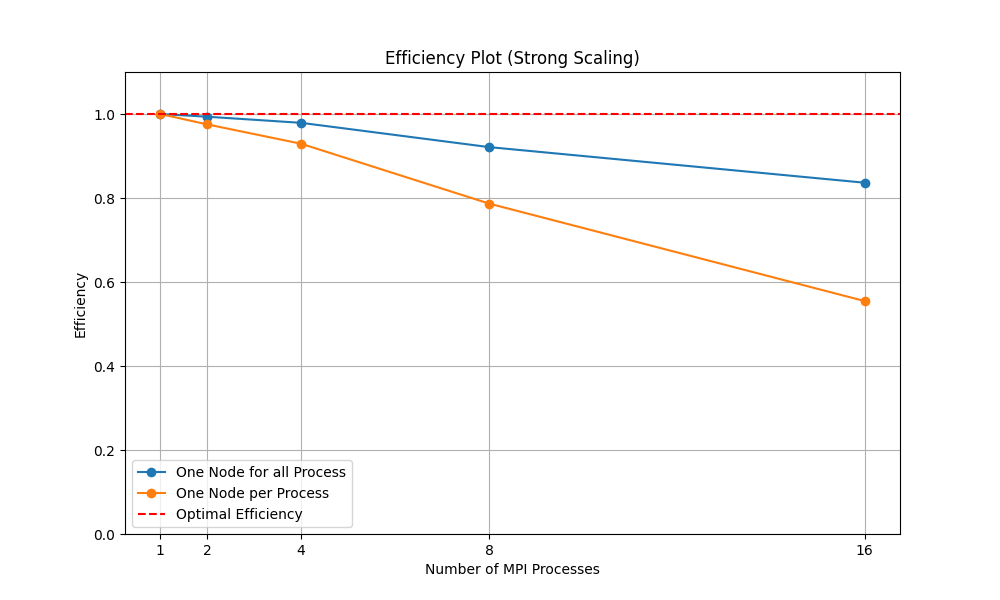
\includegraphics[width=\textwidth]{../media/efficiency_plot_eff_strong.png}
	\caption{Strong scaling}
	\label{fig:strong_eff}
    \end{subfigure}
    \hfill 
    \begin{subfigure}[b]{0.8\textwidth}
        \centering
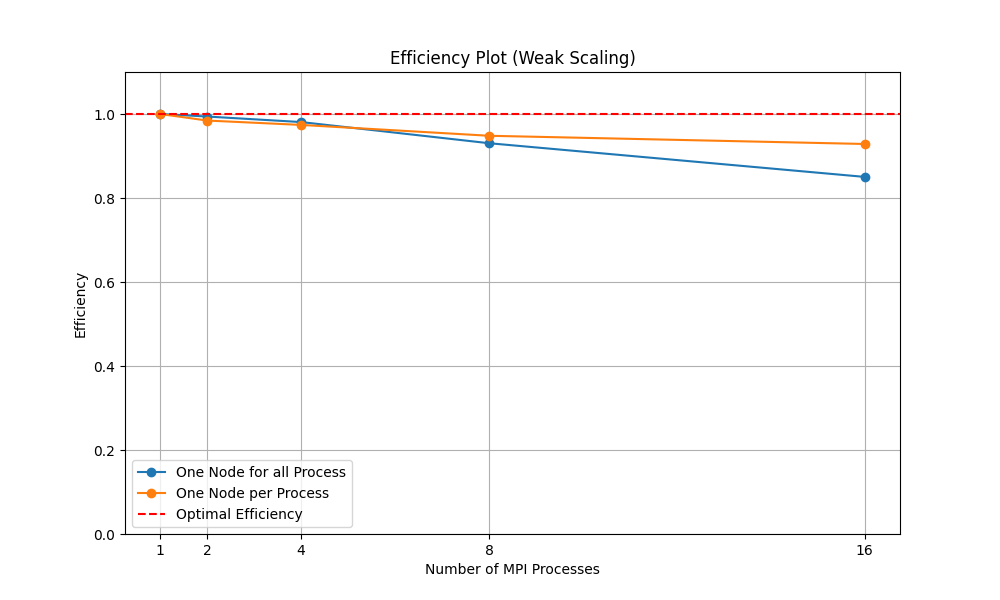
\includegraphics[width=\textwidth]{../media/efficiency_plot_eff_weak.png}
	\caption{Weak Scaling}
	\label{fig:weak_eff}
    \end{subfigure}
    \caption{Efficiency Plots for the Weak and Strong Scaling case}
    \label{fig:eff}
\end{figure}

In the strong scaling case in Subfigure \ref{fig:strong_eff}, for smaller number of processes the efficiency is relatively high and then decreases for higher number of processes due to the overhead by using more processes. The efficiency drops strong for the power method run on multiple nodes compared to the one run on a single node, this again highlights the increased overhead created when communication between multiple nodes.\newline
\newline
For the weak scaling case in Subfigure \ref{fig:weak_eff}, due to the proportionally increased workload per number of processes the efficiency is clearly better than in Strong scaling case. Due to increasing size of the matrix the overhead to workload ratio is lower, resulting in higher efficiency. Comparing the single to the multiple node, we can see that the power method run on multiple nodes is slightly more efficient, especially for a higher number of processes.
